
%----------------------------------------------------------------------------------------------------------------------
\begin{frame}{Introduction}
\begin{itemize}[noitemsep,label=\textbullet,topsep=2pt,parsep=2pt,partopsep=2pt]
\item Shapes modeled using CAD applications are used in downstream applications like,
\begin{itemize}
\item Manufacturing (Computer Aided Manufacturing , CAM),
\item Analysis (Computer Aided Engineering, CAE), etc
\end{itemize}
\item Before taking to CAE, at the earlier stage in Design, the CAD models are often simplified so that analysis gets performed with lesser resources and time.

\vspace{.5cm}
%\includegraphics[scale=0.65]{../Common/images/idealization.jpg}
\includegraphics[width=0.7\linewidth]{../Common/images/idealization.jpg}
\end{itemize}

%Notes: 

\end{frame}


%----------------------------------------------------------------------------------------------------------------------

\begin{frame}{What is Model Simplification?}
\begin{itemize}[noitemsep,label=\textbullet,topsep=2pt,parsep=2pt,partopsep=2pt]
\item 'Model Simplification' mainly involves removal of irrelevant features (De-featuring) and idealizing solids to surfaces/curves (Dimension Reduction).
\item Midsurface extraction is one of the ways of the Dimension Reduction technique where thin-walled portions of a solid are idealized to surfaces.

\vspace{.5cm}
%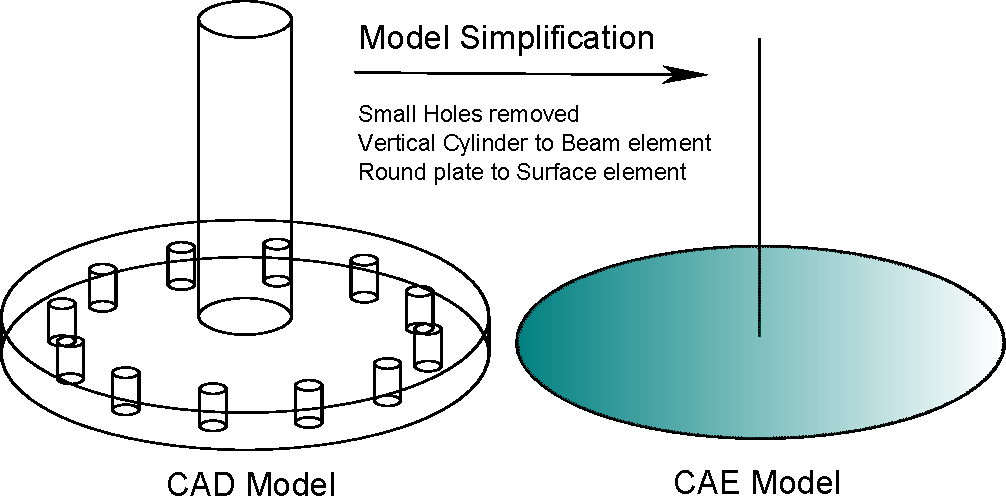
\includegraphics[scale=0.45]{../Common/images/ModelSimplification.pdf}
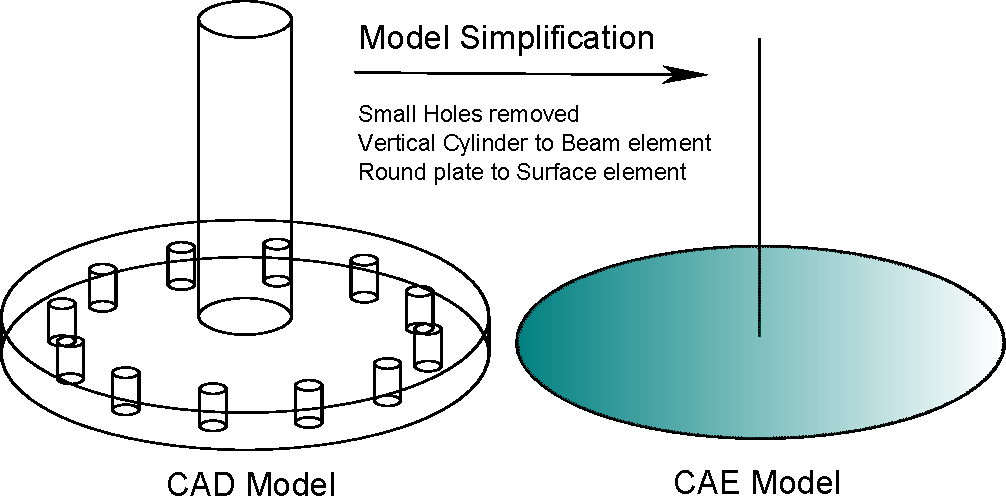
\includegraphics[width=0.85\linewidth]{../Common/images/ModelSimplification.pdf}
\end{itemize}
\end{frame}


%----------------------------------------------------------------------------------------------------------------------
\begin{frame}{What is Midsurface?}
\begin{itemize}[noitemsep,label=\textbullet,topsep=2pt,parsep=2pt,partopsep=2pt]
\item Surface approximation for the thin-walled model
\item Used to create shell element model for shell analysis
\item Not expected to work for thick models

\vspace{1cm}
%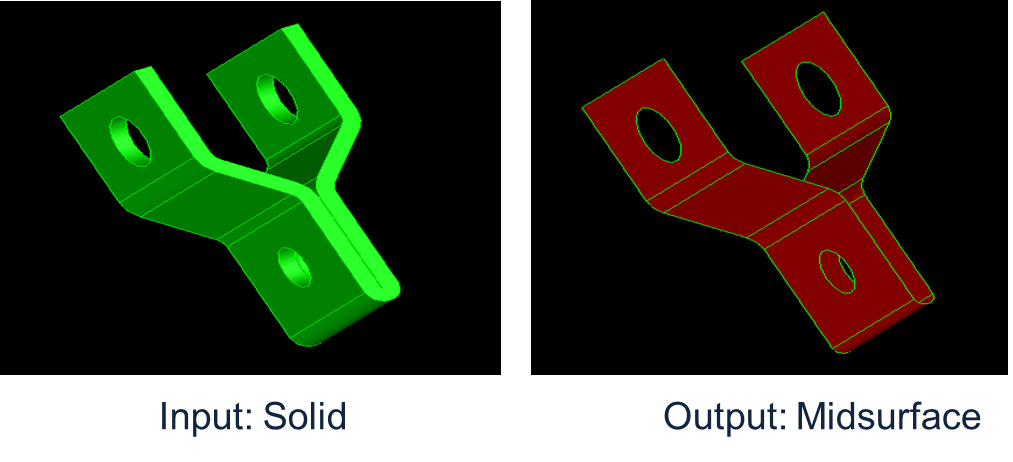
\includegraphics[scale=0.5]{../Common/images/SolidToMidsurface.png}
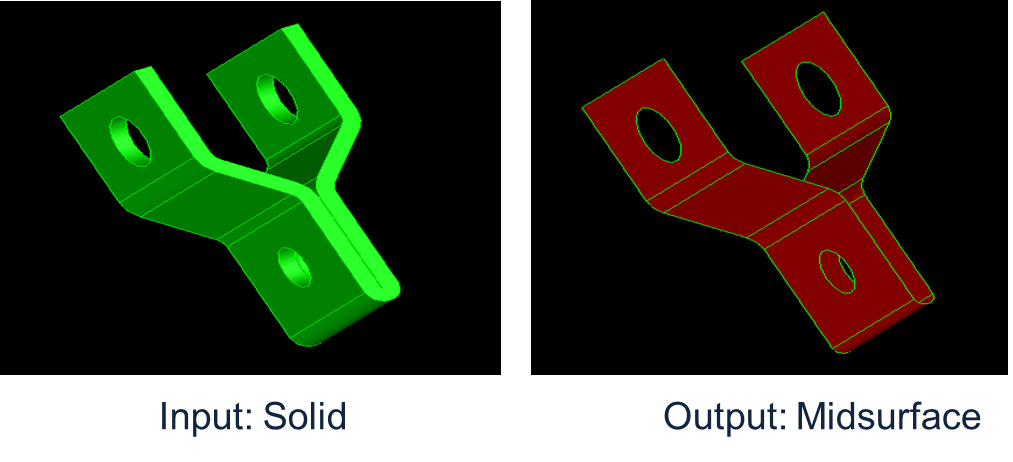
\includegraphics[width=0.85\linewidth]{../Common/images/SolidToMidsurface.png}
\end{itemize}

%Notes: 

\end{frame}
%
%%----------------------------------------------------------------------------------------------------------------------
%\begin{frame}{Where do you find Thin Wall models?}
%\vspace{1cm}
%
%%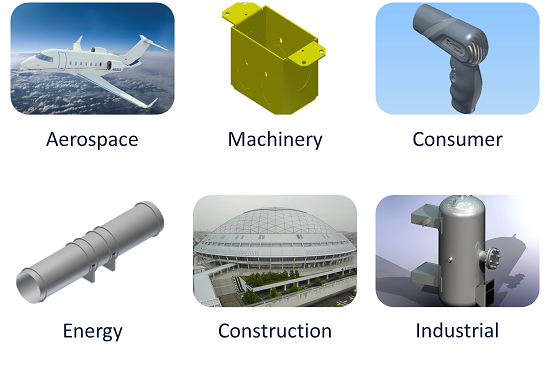
\includegraphics[scale=0.5]{../Common/images/ThinWallApplications.png}
%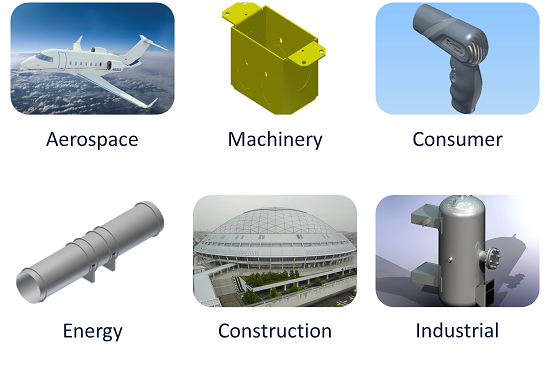
\includegraphics[width=0.85\linewidth]{../Common/images/ThinWallApplications.png}
%
%%Notes: 
%
%\end{frame}
%
%
%%----------------------------------------------------------------------------------------------------------------------
%\begin{frame}{What is considered as {\bf Thin}?}
%It is defined as a part or body with large effective span to  thickness ratio ($L/T$)
%
%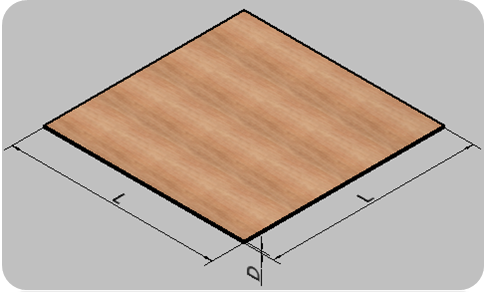
\includegraphics[scale=0.25]{../Common/images/WhatIsThin.png}
%
%For 'Thin', Solid and Shell elements give comparable results
%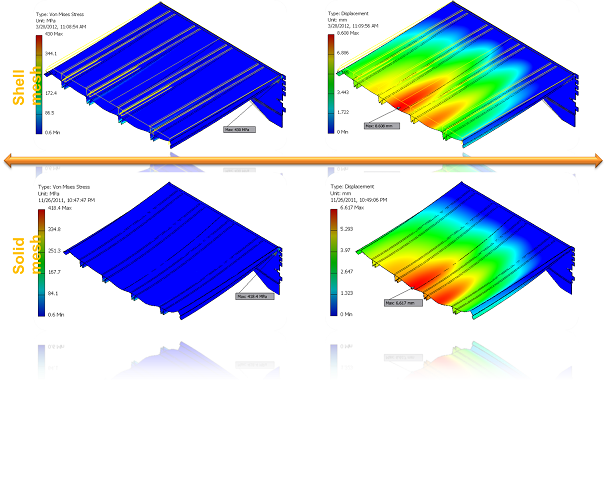
\includegraphics[scale=0.3]{../Common/images/ShellSolid.png}
%
%%Notes: 
%
%\end{frame}
%
%%
%%----------------------------------------------------------------------------------------------------------------------
%%\begin{frame}{What is considered as {\bf Thin}?}
%%It is defined as a part or body with large effective span to  thickness ratio ($L/T$)
%%
%%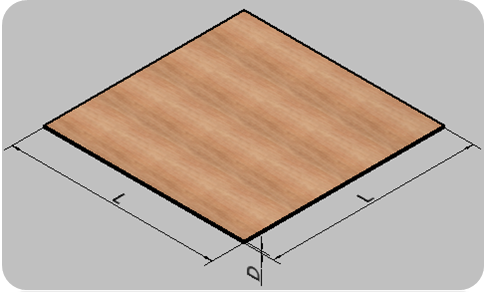
\includegraphics[scale=0.25]{../Common/images/WhatIsThin.png}
%%
%%For 'Thin', Solid and Shell elements give comparable results
%%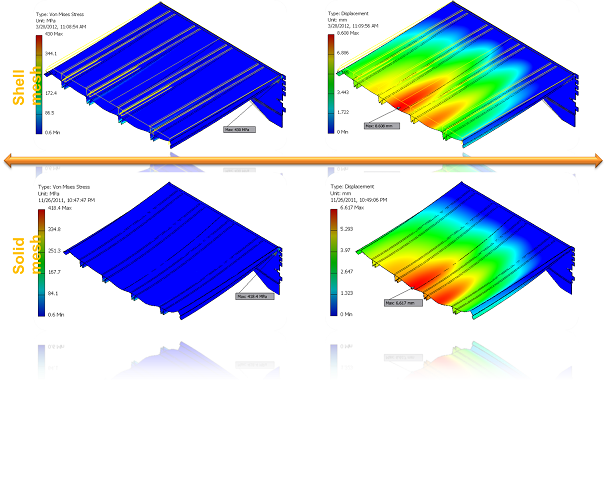
\includegraphics[scale=0.3]{../Common/images/ShellSolid.png}
%%
%%%Notes: 
%%
%%\end{frame}
%
%%----------------------------------------------------------------------------------------------------------------------
%%
%\begin{frame}{Classification of Thin-ness}
%Thickness threshold is based on the Length to Thickness ratio  $L/T$ 
%
%\begin{itemize}
%\item Length = Overall length of the input solid body
%\item Thickness = Thickness of the input solid body
%\end{itemize}
%%\begin{table}[!h]
%\begin{tabular}[h]{@{}l l l  @{}}
%\toprule
%
%{\bf $L/T$  ratio } & {\bf Interpretation } & {\bf Element}\\
%\midrule
%$L/T < 100$ & Body is thick & Solid \\
%$L/T \geq 100$ \& $L/T \leq 250$ & Body may be thin & Shell or Solid \\
%$L/T > 250$ \& $L/T \leq 750$ & Body is thin & Shell \\
%$L/T > 750$ & Body is too thin & Certainly Shell \\
%\bottomrule
%\end{tabular}
%%\end{table}
%
%
%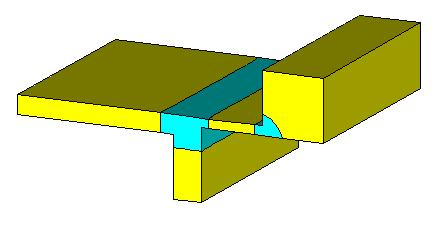
\includegraphics[scale=0.4]{../Common/images/PriceThin.jpg}
%
%\end{frame}
%
%
%%----------------------------------------------------------------------------------------------------------------------
%
%\begin{frame}{But why not just one side of it?}
%\begin{itemize}
%\item Midsurface is needed to follow shape of the base part as well as carry thickness information. It should not be biased towards one of the sides.
%\item Figure shows two configurations for 'L' shape. Irrespective of the way they have been joined, CAE would like to have surface that would follow the base part shape and look like proper 'L'. If any of the sides are taken, results are skewed.
%
%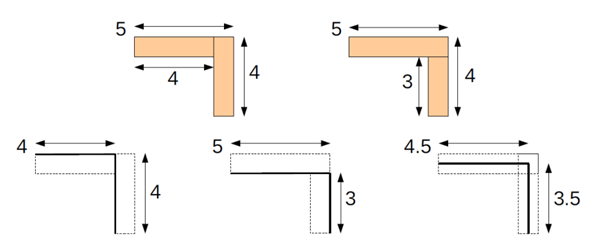
\includegraphics[scale=0.5]{../Common/images/OneSide.png}
%
%\end{itemize}
%
%%Notes: 
%
%\end{frame}
%
%%----------------------------------------------------------------------------------------------------------------------
%
%\begin{frame}{Effect of Thickness on Side-ness}
%\begin{itemize}
%\item Shell elements are meshed on surfaces (compared to solids in volumes)
%\item COSMOS [SolidWorks] understands the shell placement to ALWAYS be at the Midsurface of the part
%\begin{itemize}
%\item For convenience, it may be easier to choose an inside or outside part surface
%\item The higher the part aspect ratio, the less it matters
%\end{itemize}
%
%\vspace{0.5cm}
%
%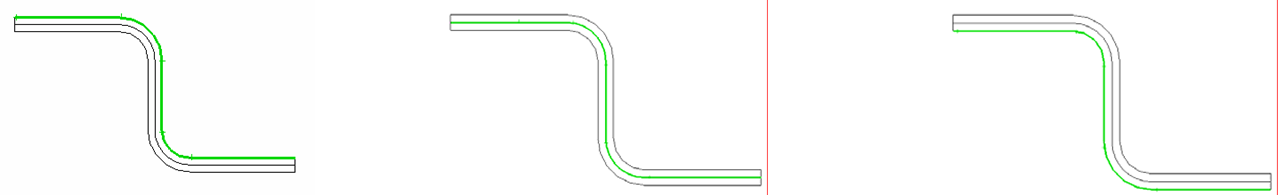
\includegraphics[scale=0.45]{../Common/images/EffectOfThickness.png}
%
%\end{itemize}
%
%\end{frame}
%
%

%----------------------------------------------------------------------------------------------------------------------
%
%\begin{frame}{Methods for Midsurface computation}
%\begin{itemize}
%\item Midsurface Abstraction (MA) Approach and Medial Axis Transform (MAT) Approach are based on Extraction, meaning the algorithm is applied on the ready-final model to extract Midsurface. 
%
%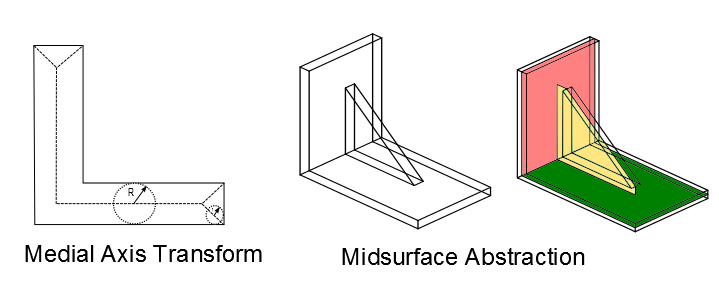
\includegraphics[scale=0.25]{../Common/images/MAT_Midsurf.png}
%
%\item Many a times due to complexity in recognizing forms, their interactions, same design-intent used while modeling part can not be applied to Midsurface and thus Midsurface of part does not follow its form and connectivity
%
%\item Idea is to leverage the design intent in the form of feature history tree, to build the Midsurface as the way model gets built, step by step.
%\end{itemize}
%
%%Notes: 
%
%\end{frame}
%%
%%----------------------------------------------------------------------------------------------------------------------
%
%\begin{frame}{When-What}
%\begin{itemize}
%\item \textbf{1967} Blum: MAT
%\item \textbf{1994} Dabke: Features for Idealization
%\item \textbf{1996} Armstrong: MAT for CAE
%\item \textbf{1996} Rezayat: MA SDRC
%\item \textbf{1999} Fischer: Parametric Midcurves
%\item \textbf{2002} Deng: FBD Simplification
%\item \textbf{2005} Stolt: Pocket Pad based Midsurface
%\item \textbf{2007} Robinson: Sketch based Midsurface
%\item \textbf{2012} Russ: FBD defeaturing
%\item \textbf{2013} Woo: Decomp, per feature Midsurface
%\end{itemize}
%
%%Notes: 
%
%\end{frame}

%%----------------------------------------------------------------------------------------------------------------------
%\begin{frame}{Literature Survey Conclusions}
%\begin{itemize}
%\item Model Simplification is essential even when computation power has increased dramatically \cite{Stolt2005}, because:
%	\begin{itemize}
%	\item more complex problems can be solved
%	\item more design iterations can be performed
%	\end{itemize}
%
%\item Medial generation method?
%	\begin{itemize}
%	\item MAT: unsuitable as it creates branches
%	\item MA: Face pairing is complex
%	\item Feature based: So far Sweep based and primitives have been tried. No one, so far has worked on feature interactions, extend-trim and non-manifold boolean to get connected Midsurface
%	\end{itemize}

%\item Which Domain? [Nitish Sand Interview]
%	\begin{itemize}
%	\item Injection Molding parts are most complex due to draft and have most demand 
%	\item Sheet Metal parts are relatively easy, create surfaces but fail in connections. 
%	\item Start with Sheet Metal parts and then attempt generic or injection molding parts
%	\end{itemize}
%
%\item {\em There is a definite need for a dimensional reduction capability that is more powerful and easier to use than those currently available in the market. Such a capability should deliver an automated scheme for handling cases that have traditionally caused problems for algorithms in this field} \cite{Stanley2010}
%%
%%\item {\em Much of research is yet to be done, use of symmetry, various features, various abstractions are not yet handled} \cite{Smit2011}
%
%\end{itemize}
%
%%Notes: 
%
%\end{frame}

%----------------------------------------------------------------------------------------------------------------------
\begin{frame}{Problems Identified so far}
\vspace{0.8cm}
%\centering 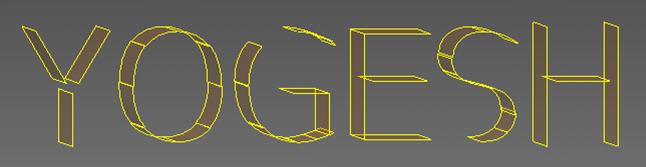
\includegraphics[scale=0.5]{../Common/images/YOGESH_Midsurf.png}
\centering 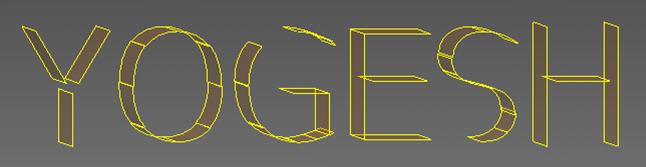
\includegraphics[width=0.85\linewidth]{../Common/images/YOGESH_Midsurf.png}
\end{frame}

%
\begin{frame}{Benchmarking Software used...}
\begin{itemize}[noitemsep,label=\textbullet,topsep=2pt,parsep=2pt,partopsep=2pt]

\item Got results from 


\includegraphics[width=0.3\linewidth]{../Common/images/Logo_AutodeskInventor}
\vspace{5mm}

\includegraphics[width=0.3\linewidth]{../Common/images/Logo_PTC}

\includegraphics[width=0.3\linewidth]{../Common/images/Logo_Altair}

\item Yet to get access to

\vspace{5mm}
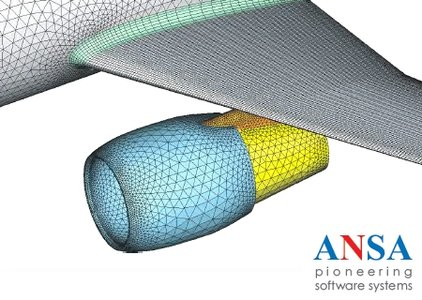
\includegraphics[width=0.3\linewidth]{../Common/images/Logo_Ansa.jpeg}
\vspace{35mm}

\includegraphics[width=0.3\linewidth]{../Common/images/Logo_PamStamp}


\end{itemize}
%Notes: 
\end{frame}
%----------------------------------------------------------------------------------------------------------------------
\begin{frame}{Basic Shape: T}
\begin{itemize}[noitemsep,label=\textbullet,topsep=2pt,parsep=2pt,partopsep=2pt]

\item Inventor Auto Midsurface

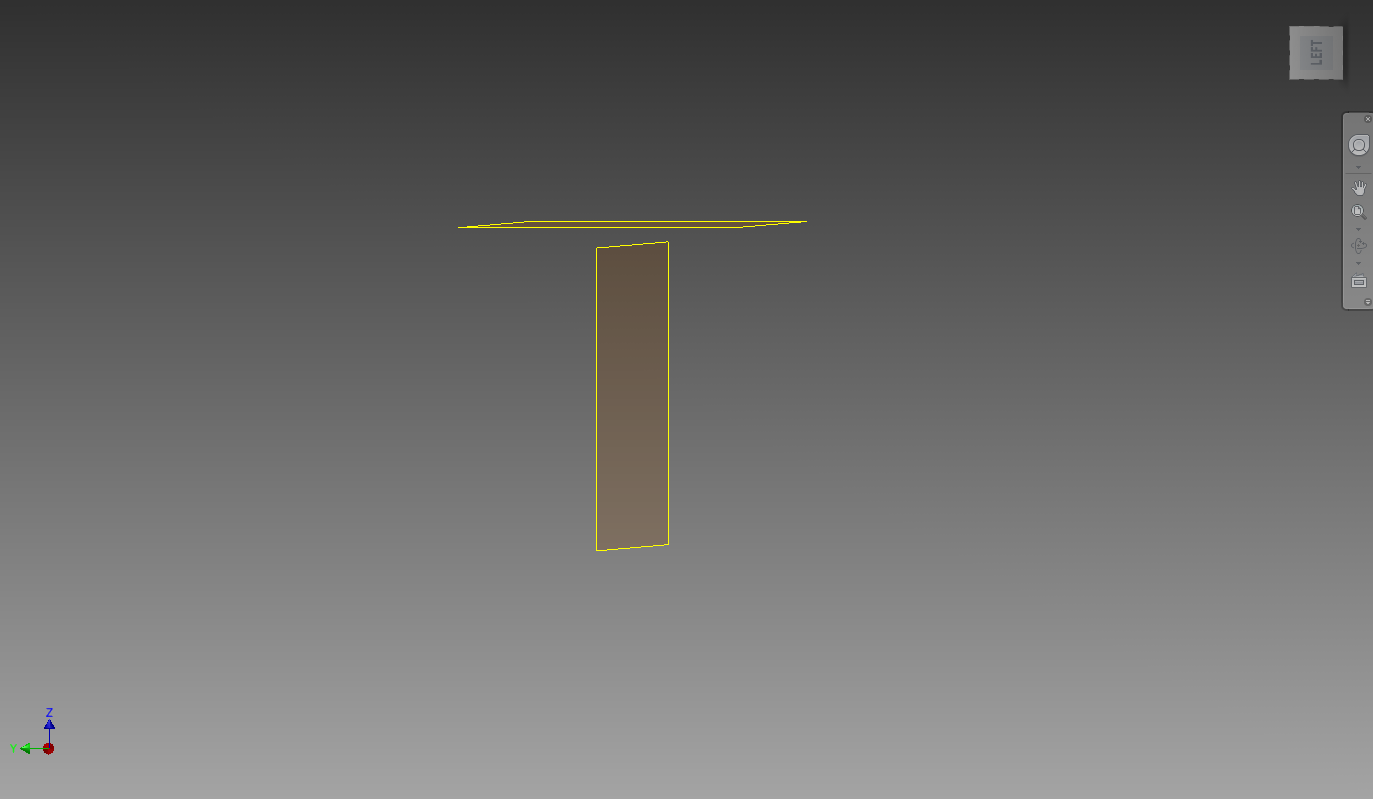
\includegraphics[scale=0.09]{../Common/images/Inventor_T_Mids.png}

\item Pro/E Auto Midsurface

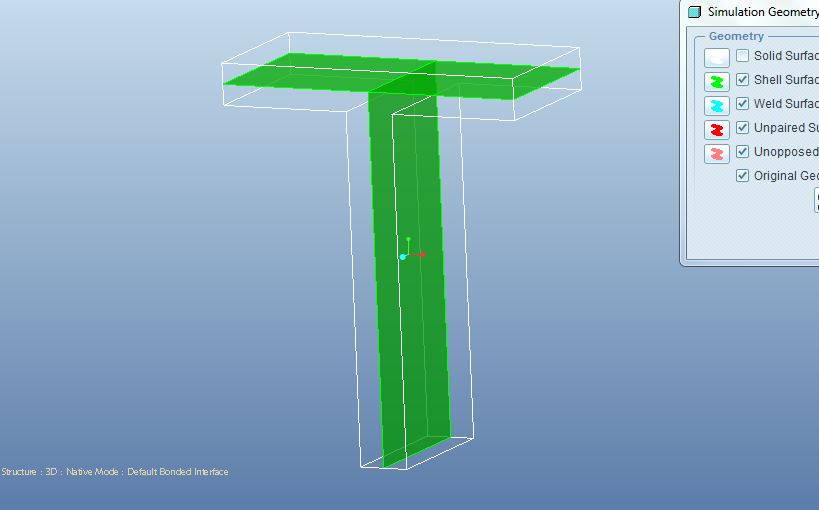
\includegraphics[scale=0.15]{../Common/images/ProeTautoPairs.png}

\item Hypermesh Auto Midsurface

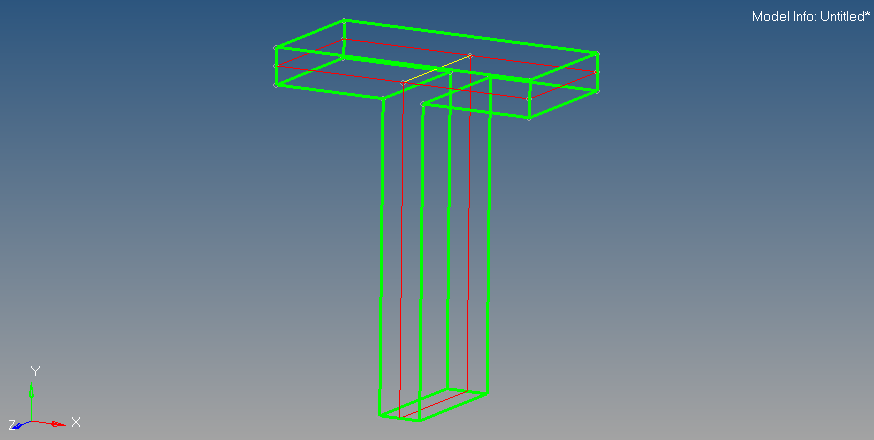
\includegraphics[scale=0.18]{../Common/images/HypermeshTauto.png}

\item \textcolor{green}{ProE and Hypermesh are good!!}
\end{itemize}
%Notes: 
\end{frame}
%----------------------------------------------------------------------------------------------------------------------

%----------------------------------------------------------------------------------------------------------------------
\begin{frame}{Basic Shape: H}
\begin{itemize}[noitemsep,label=\textbullet,topsep=2pt,parsep=2pt,partopsep=2pt]

\item Inventor Auto Midsurface

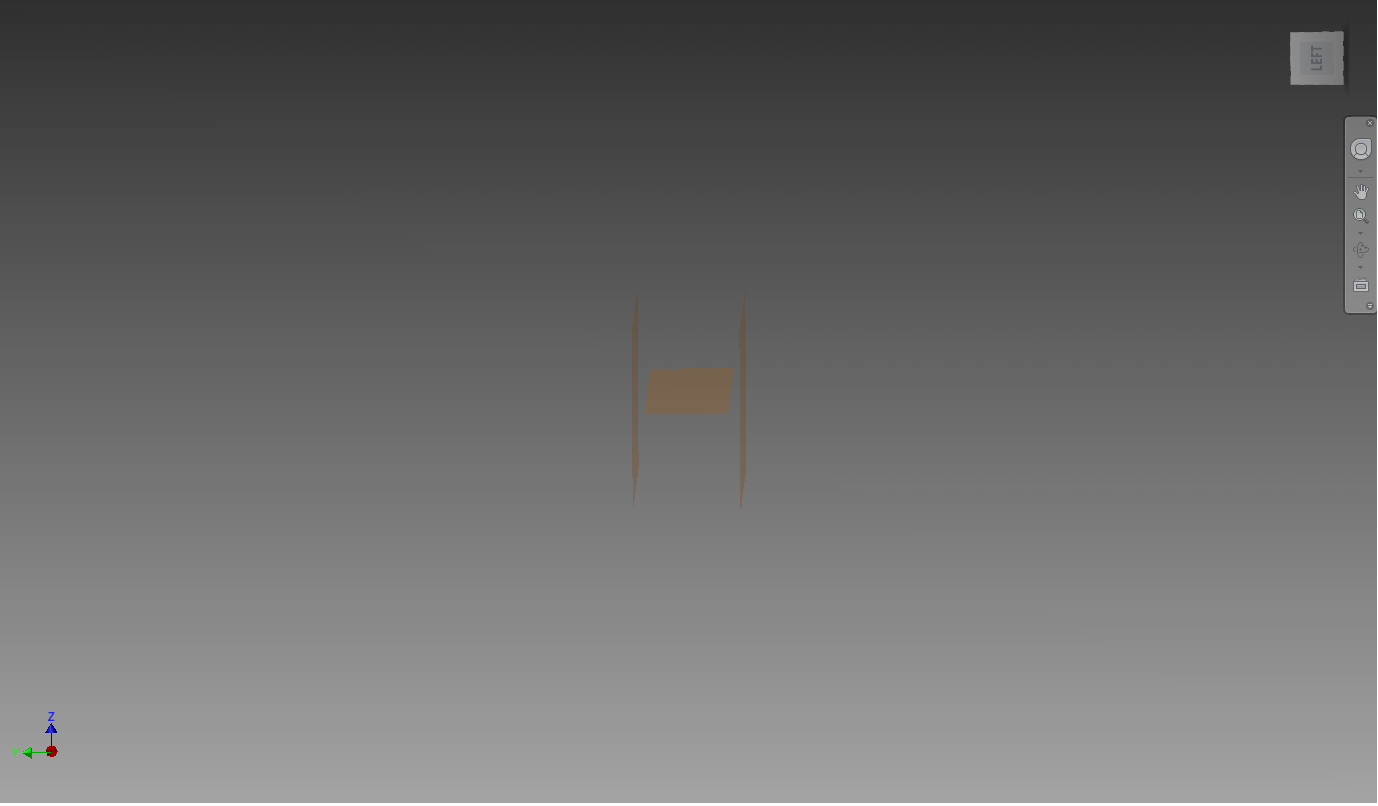
\includegraphics[scale=0.11]{../Common/images/Inventor_H_Mids.png}

\item Pro/E Auto Midsurface

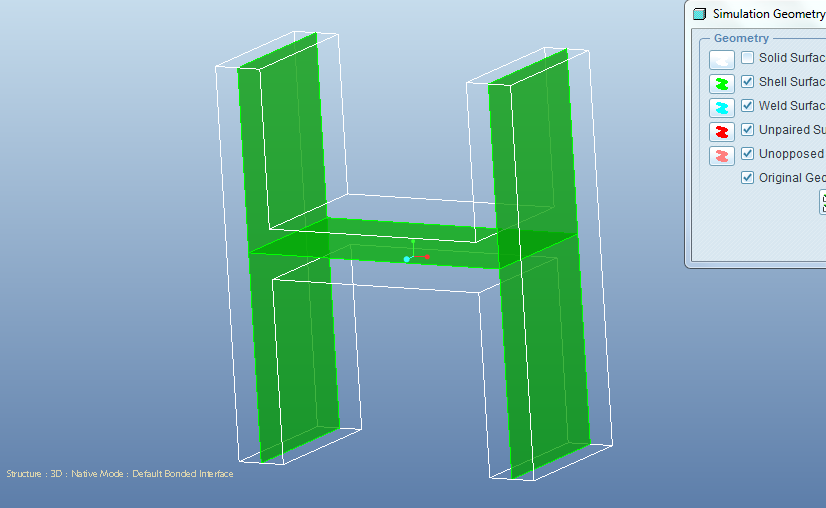
\includegraphics[scale=0.15]{../Common/images/ProeHautoPairs.png}

\item Hypermesh Auto Midsurface

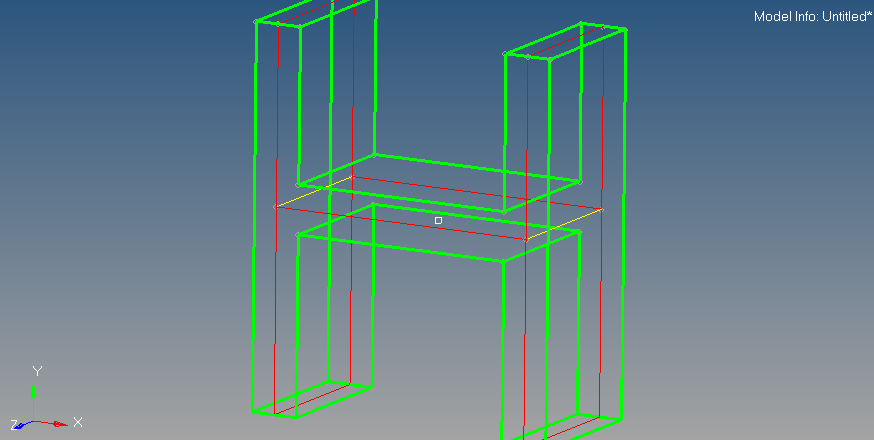
\includegraphics[scale=0.18]{../Common/images/HypermeshHauto.png}

\item \textcolor{green}{ProE and Hypermesh are good!!}
\end{itemize}
%Notes: 
\end{frame}
%----------------------------------------------------------------------------------------------------------------------

%----------------------------------------------------------------------------------------------------------------------
\begin{frame}{Basic Shape: K}
\begin{itemize}[noitemsep,label=\textbullet,topsep=2pt,parsep=2pt,partopsep=2pt]

\item Inventor Auto Midsurface

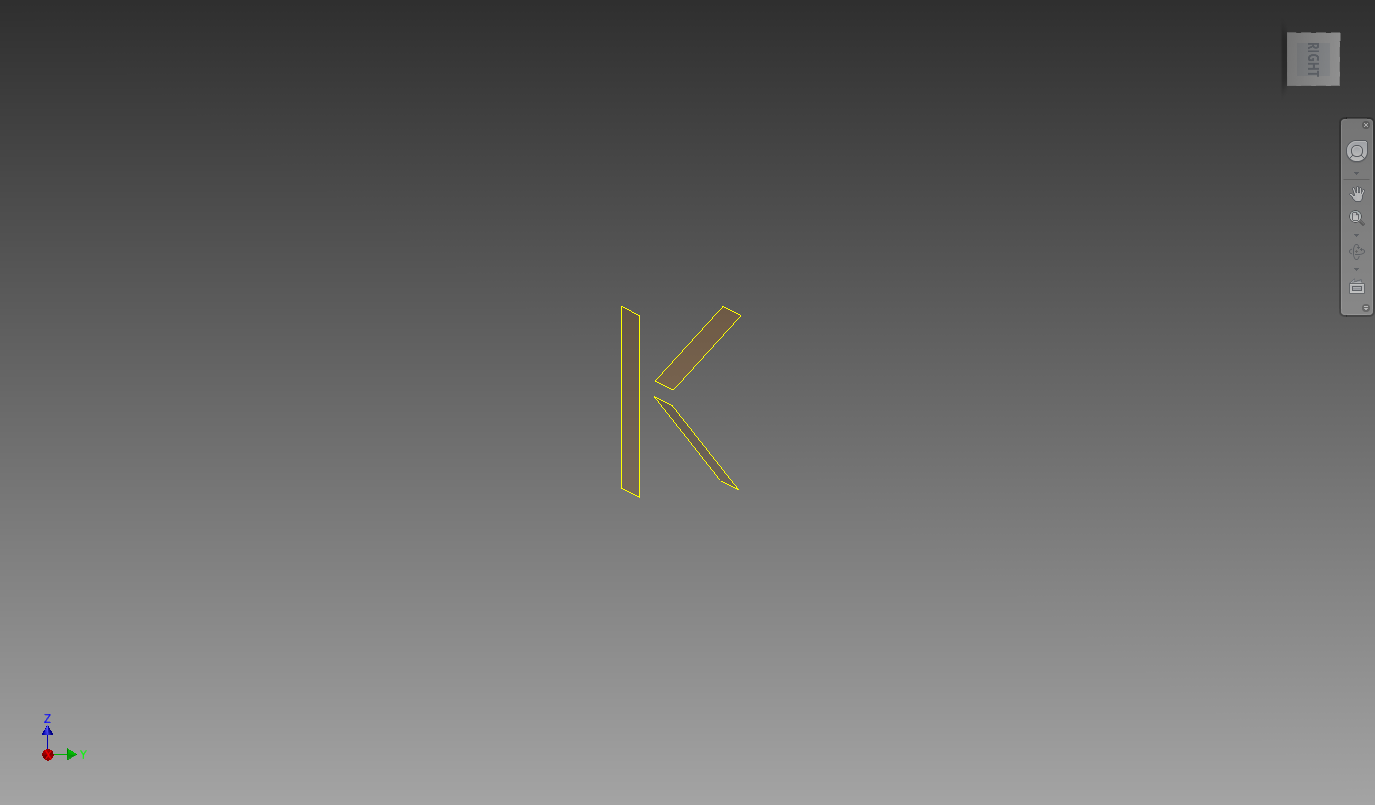
\includegraphics[scale=0.11]{../Common/images/Inventor_K_Mids.png}

\item Pro/E Auto Midsurface

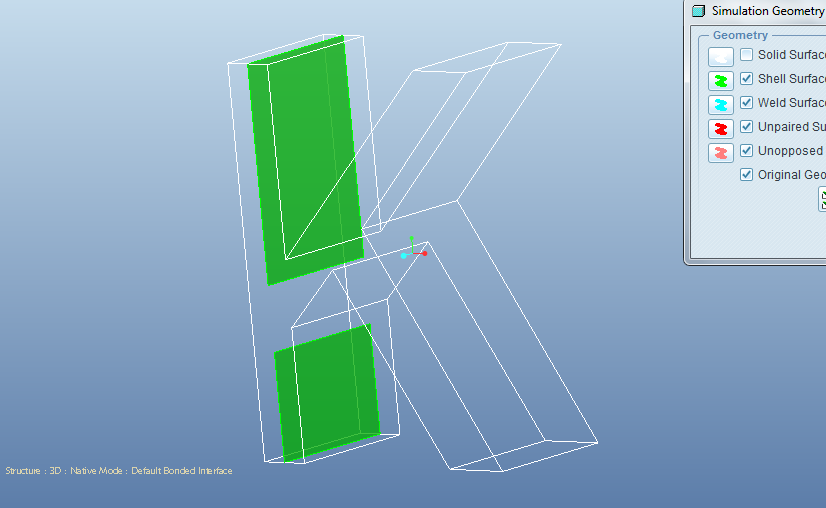
\includegraphics[scale=0.15]{../Common/images/ProeKautoPairs.png}

\item Hypermesh Auto Midsurface

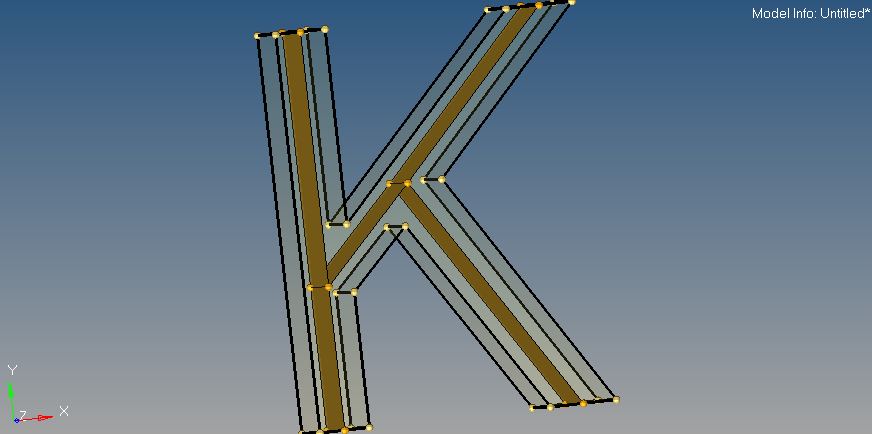
\includegraphics[scale=0.18]{../Common/images/HypermeshKauto.png}

\item \textcolor{green}{Only Hypermesh is good!!}
\end{itemize}
%Notes: 
\end{frame}
%----------------------------------------------------------------------------------------------------------------------

%----------------------------------------------------------------------------------------------------------------------
\begin{frame}{Basic Shape: Y}
\begin{itemize}[noitemsep,label=\textbullet,topsep=2pt,parsep=2pt,partopsep=2pt]

\item Inventor Auto Midsurface

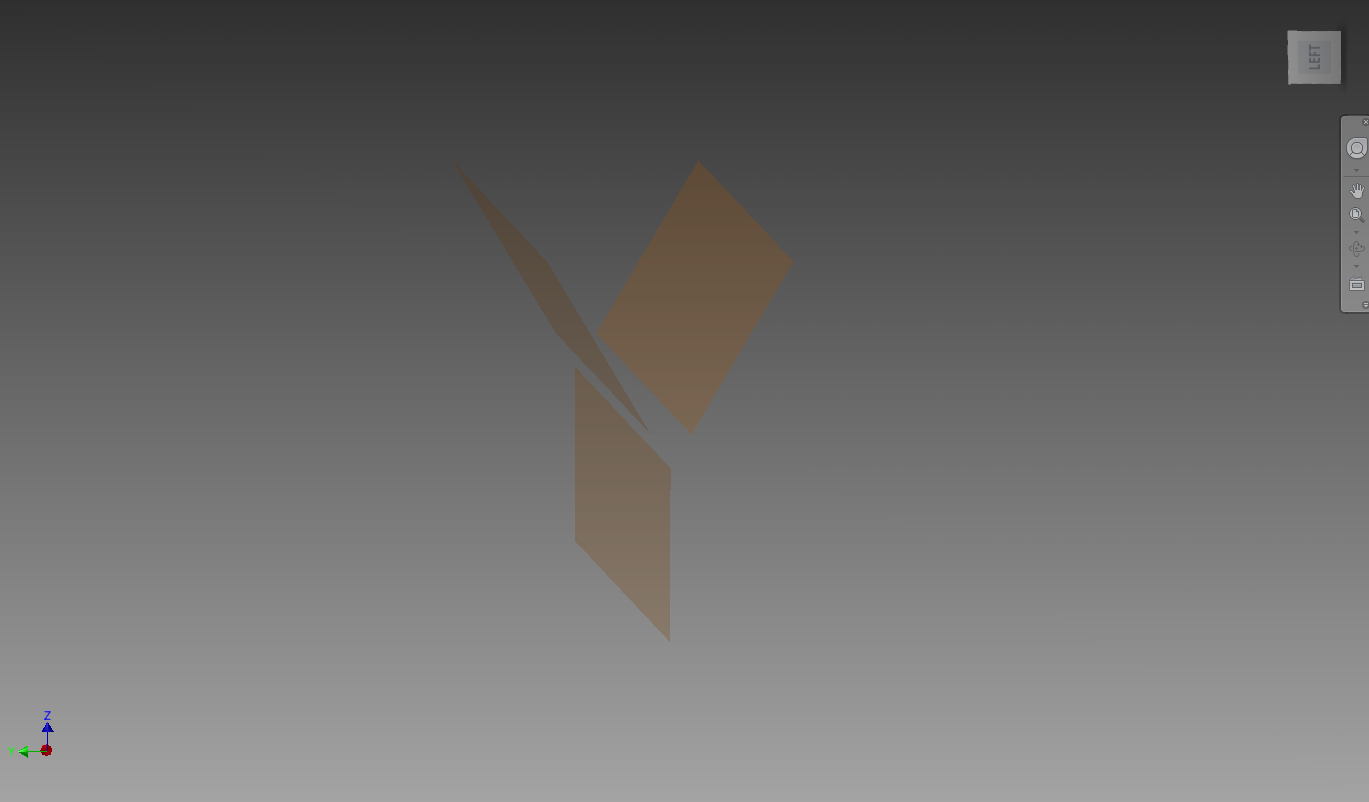
\includegraphics[scale=0.09]{../Common/images/Inventor_Y_Mids.png}

\item Pro/E Auto Midsurface

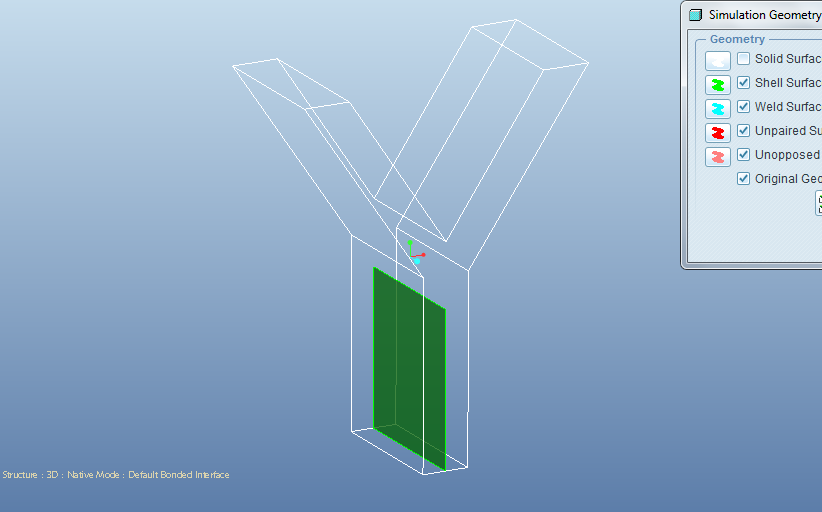
\includegraphics[scale=0.15]{../Common/images/ProeYautoPairs.png}

\item Hypermesh Auto Midsurface

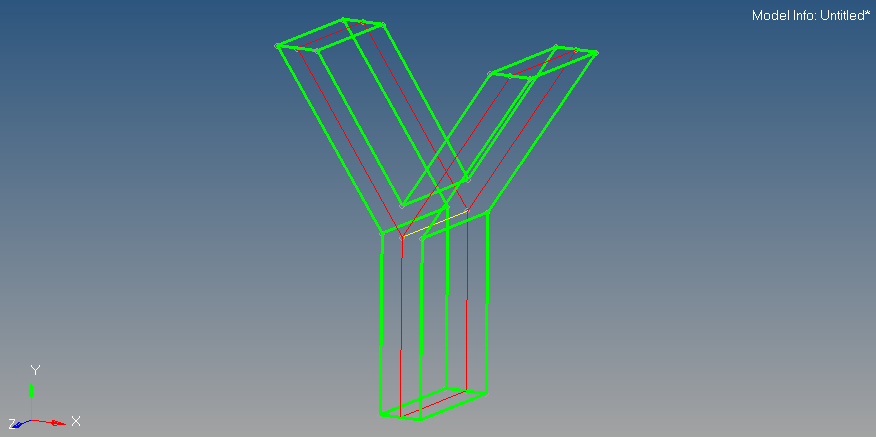
\includegraphics[scale=0.18]{../Common/images/HypermeshYauto.png}

\item \textcolor{green}{Only Hypermesh is good!!}
\end{itemize}
%Notes: 
\end{frame}
%----------------------------------------------------------------------------------------------------------------------

%----------------------------------------------------------------------------------------------------------------------
\begin{frame}{Basic Part: Wall Bracket}
\begin{itemize}[noitemsep,label=\textbullet,topsep=2pt,parsep=2pt,partopsep=2pt]

\item Inventor Auto Midsurface

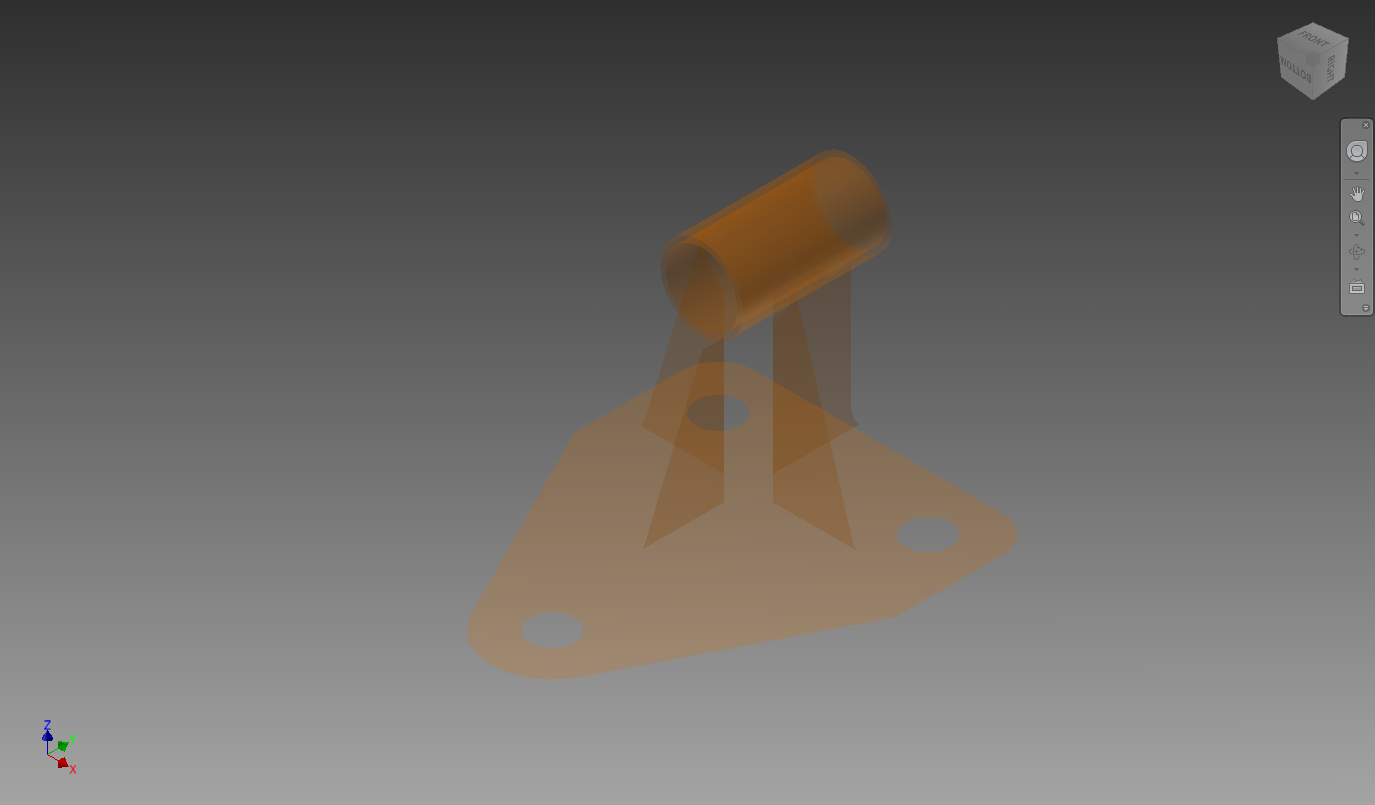
\includegraphics[width=0.5\linewidth]{../Common/images/InventorWallBracketMids.png}

\item Hypermesh Auto Midsurface

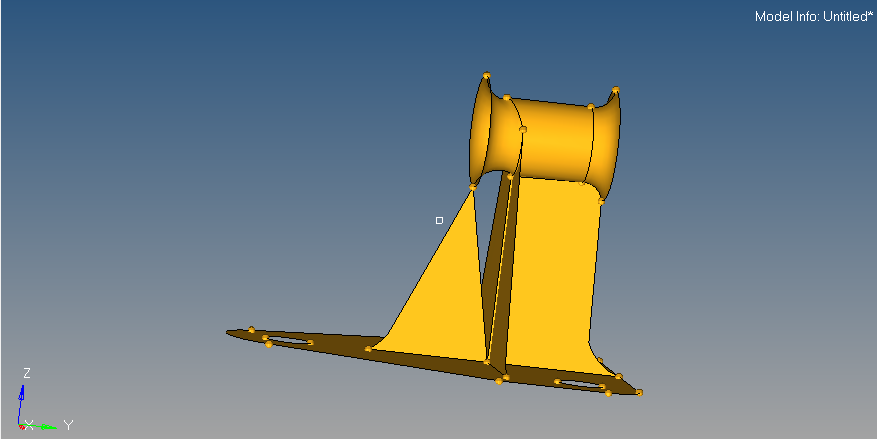
\includegraphics[width=0.5\linewidth]{../Common/images/HypermeshWallBracket.png}

\item \textcolor{red}{Even Hypermesh fails!!}
\end{itemize}
%Notes: 
\end{frame}
%----------------------------------------------------------------------------------------------------------------------

\begin{frame}{Will be using feature tree make problem simpler?}
\vspace{0.1cm}
\centering 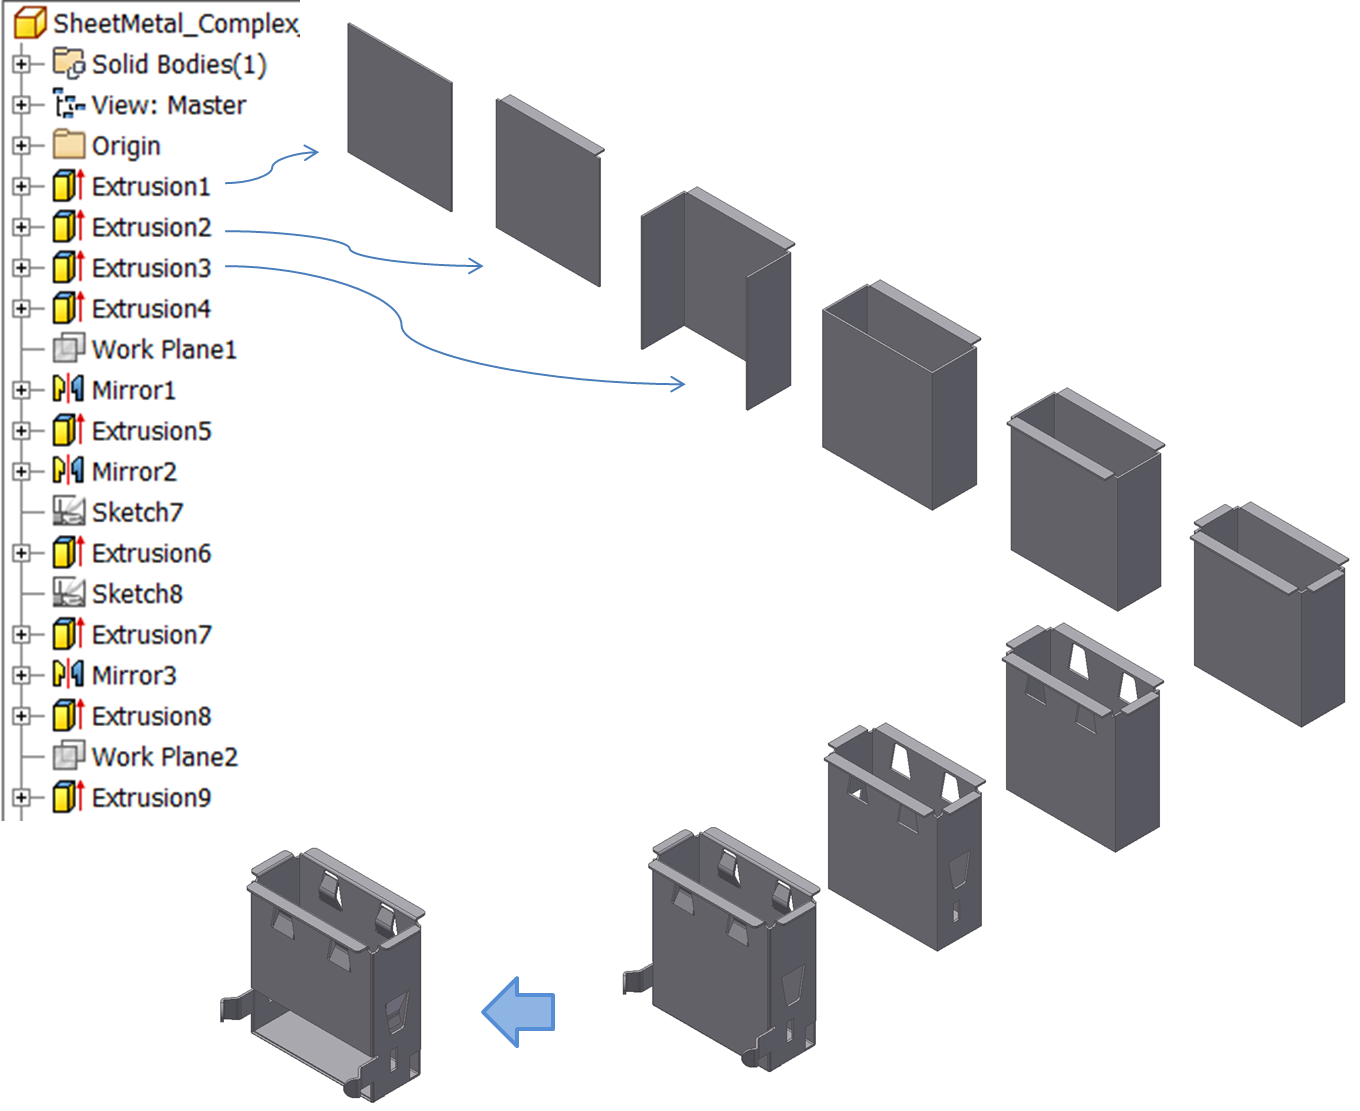
\includegraphics[height=0.7\linewidth]{../Common/images/USB_buildup}
\end{frame}
